\section{X-ray source - Three Pole Wiggler (3PW)}
\subsection{Wiggler plots}

\subsection{Source size and divergence}
Plots of the horizontal and vertical photon source size and divergence are shown in \ref{fig:3PW_source}. \\.

\begin{figure*}  % spans both columns
\begin{subfigure}{0.45\textwidth}
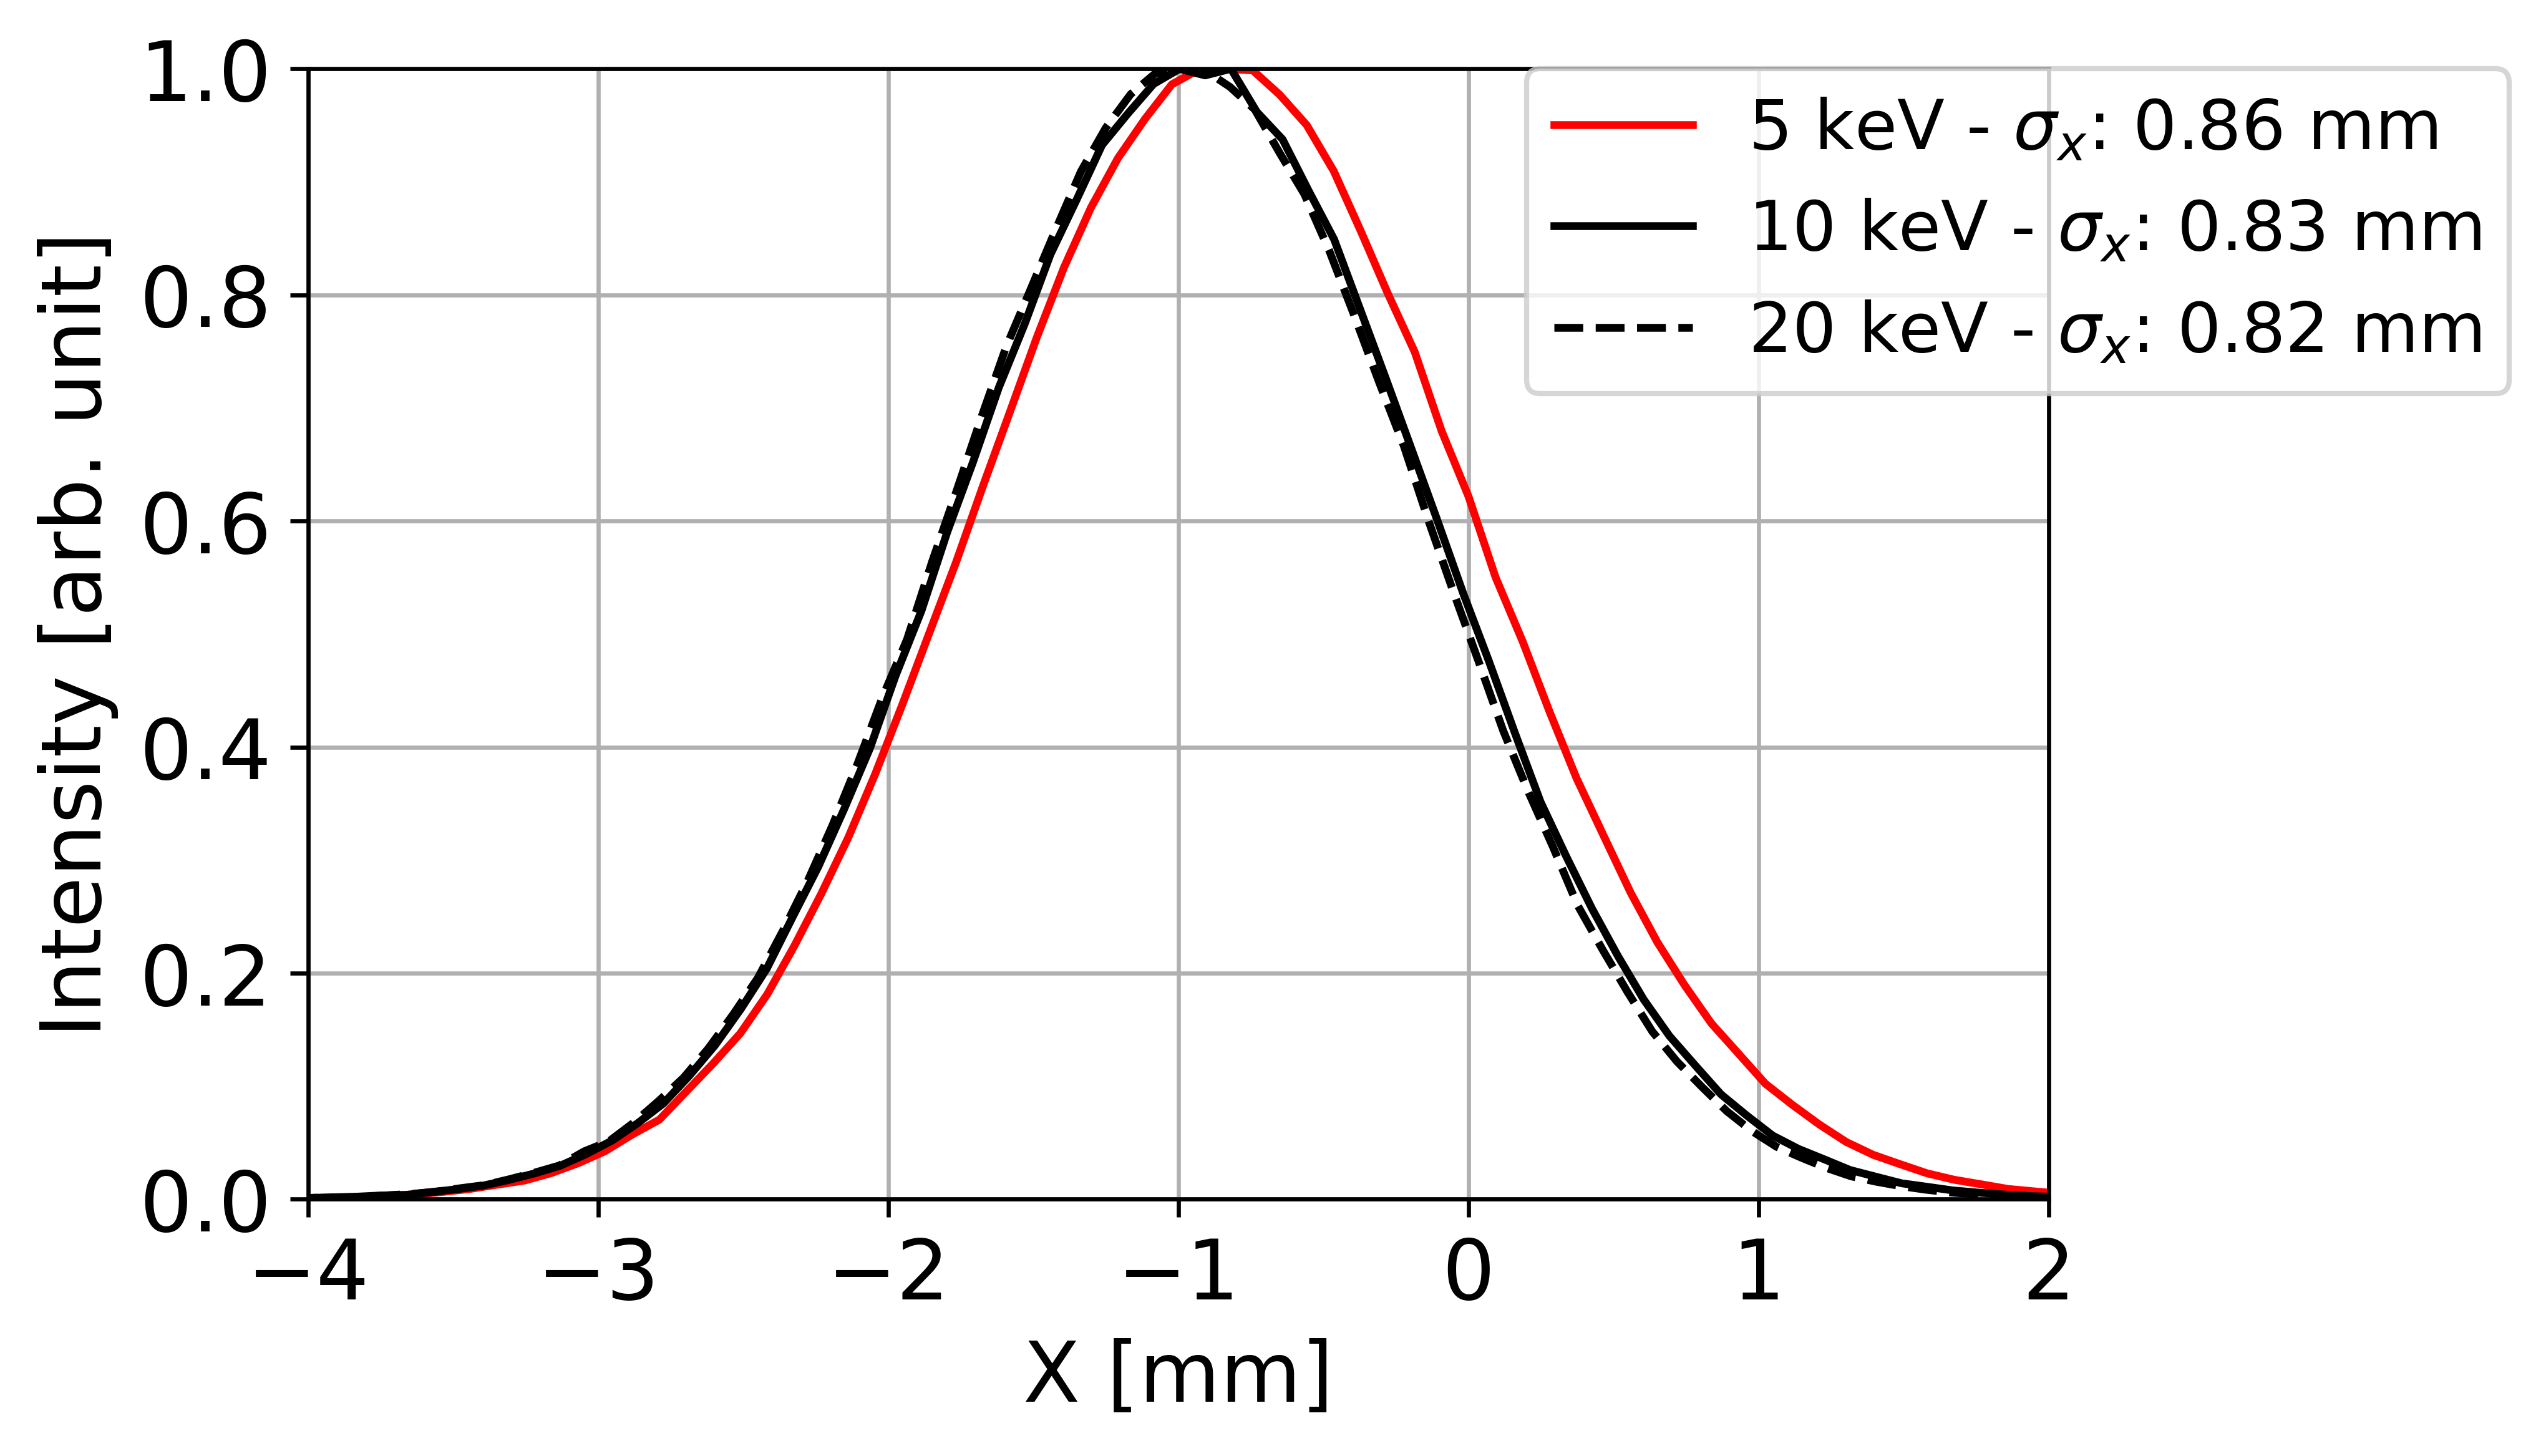
\includegraphics[width=\linewidth]{figures/beam_snapshots/3PW/sigmaX.png}
% \caption{Network 1}
\end{subfigure}
\hfill % maximize the horizontal distance between the graphs
\begin{subfigure}{0.45\textwidth}
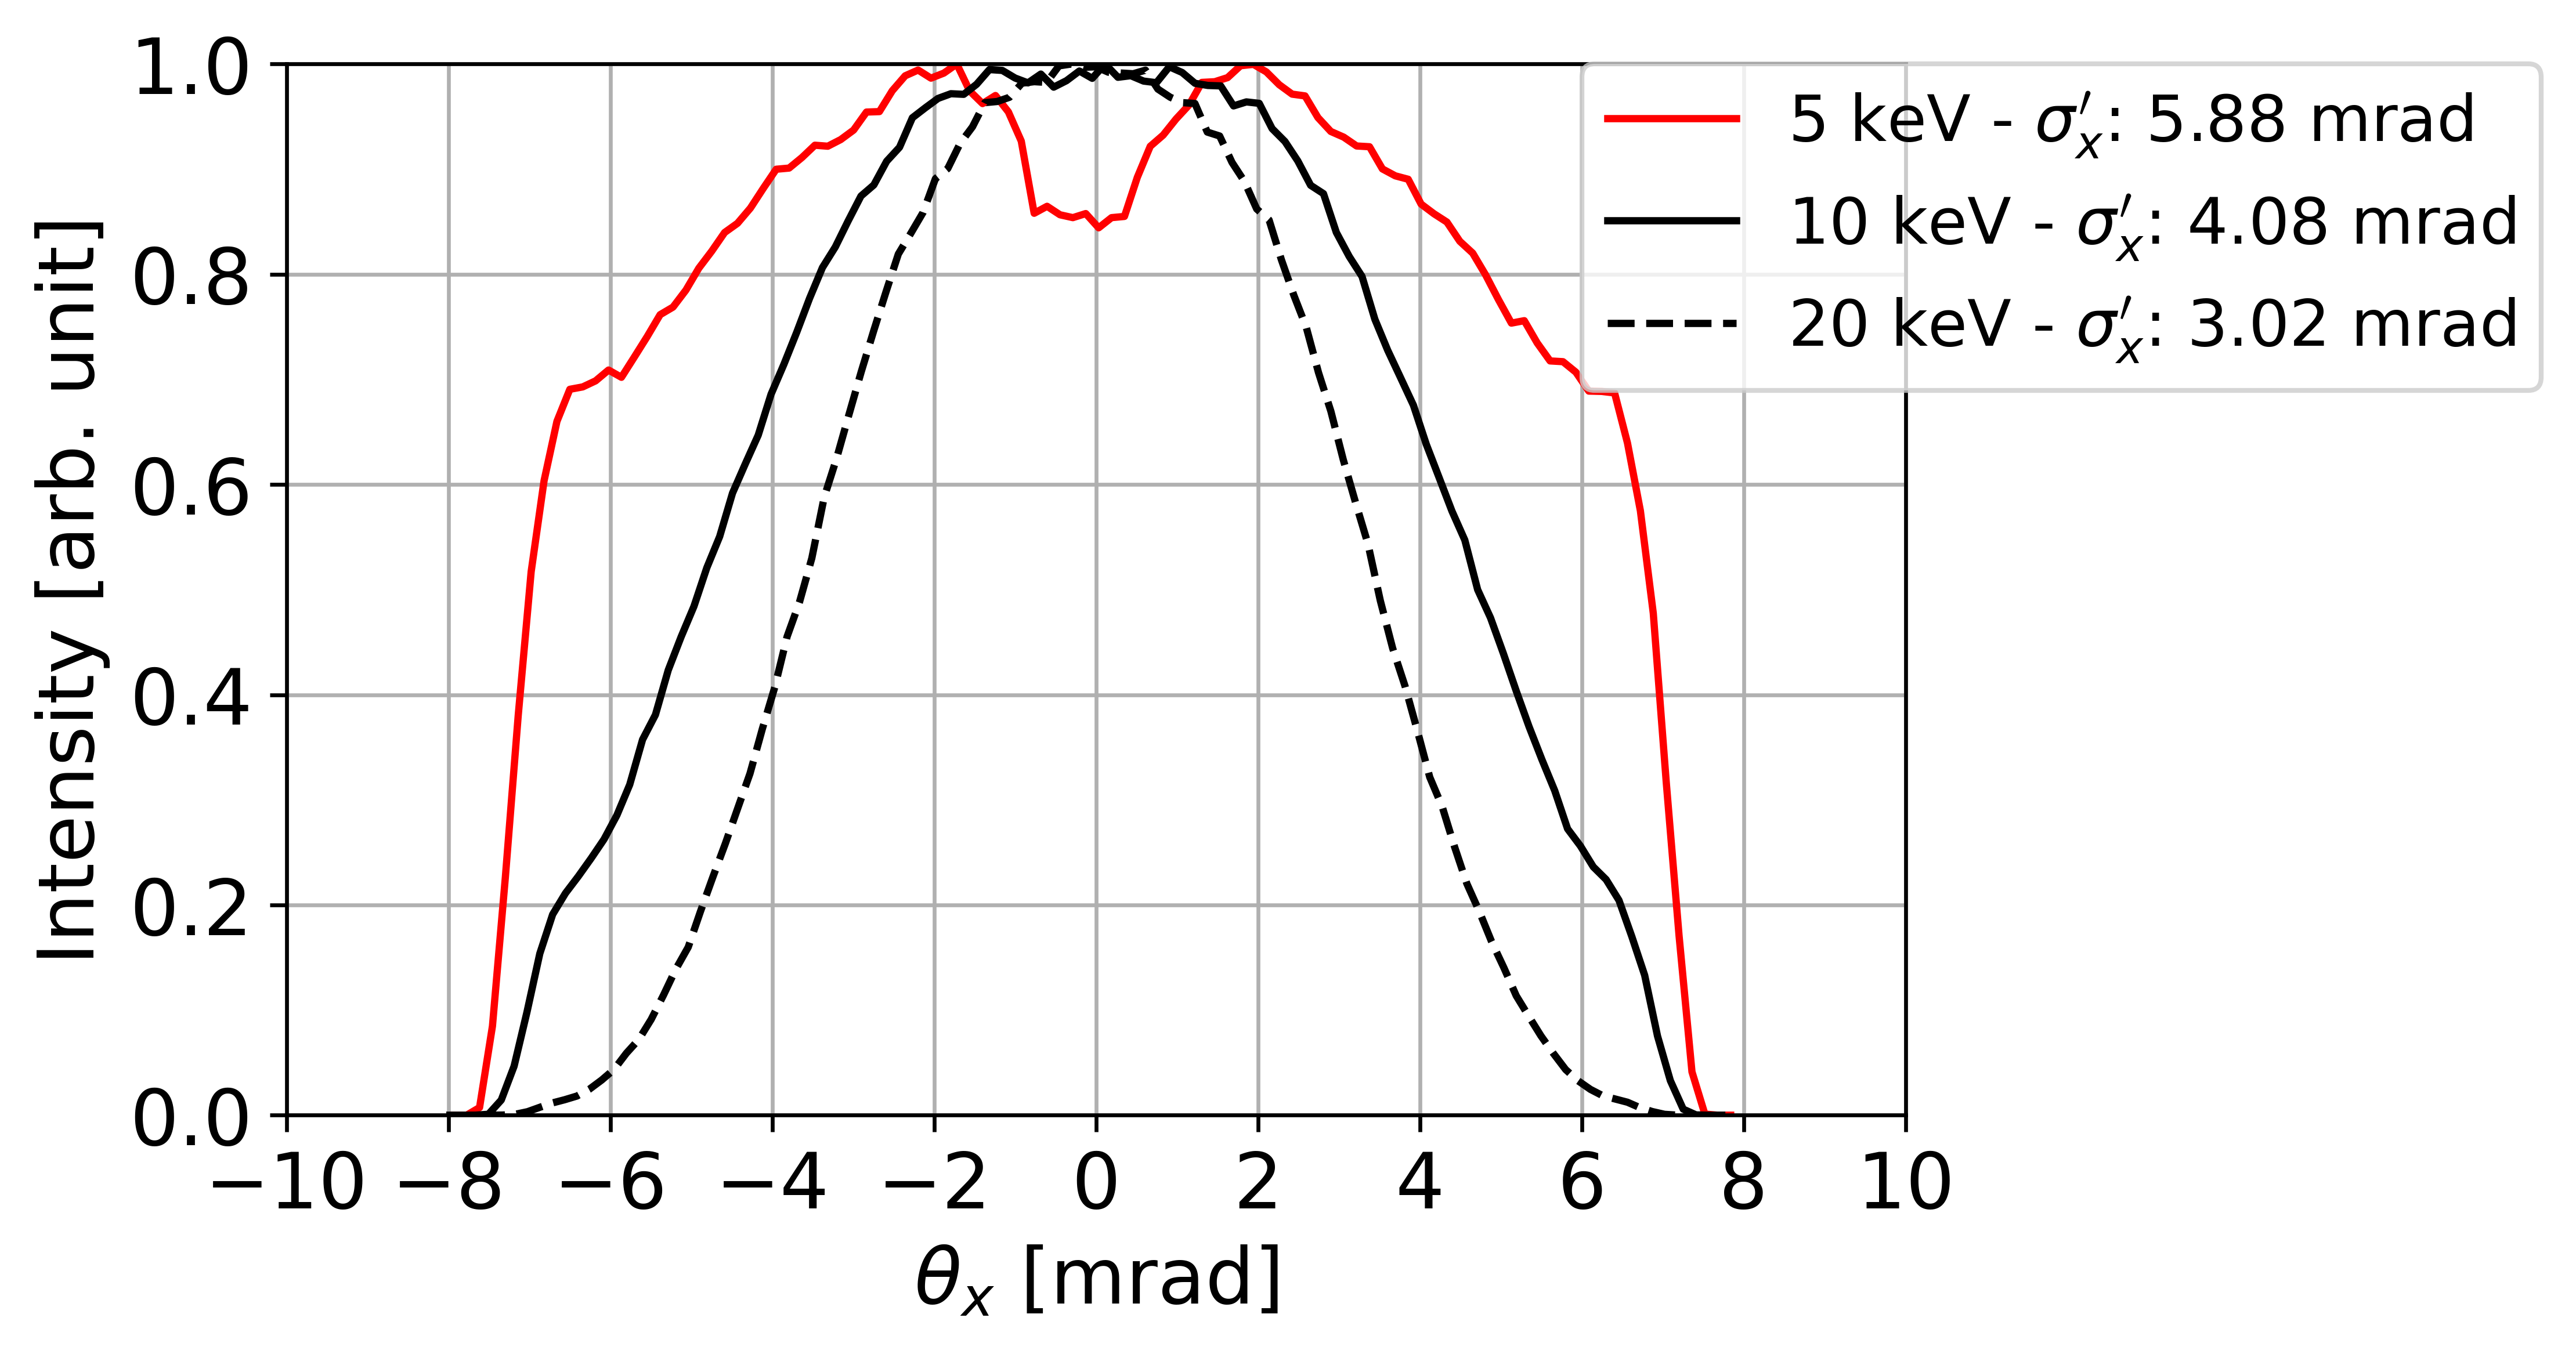
\includegraphics[width=\linewidth]{figures/beam_snapshots/3PW/sigmaXp.png}
% \caption{Network  2}
\end{subfigure}

\bigskip  % some extra vertical whitespace
\begin{subfigure}{0.45\textwidth}
\includegraphics[width=\linewidth]{c.pdf}
\caption{Network  3}
\end{subfigure}
\hfill % maximize the horizontal distance between the graphs
\begin{subfigure}{0.45\textwidth}
\includegraphics[width=\linewidth]{d.pdf}
\caption{Network  4}
\end{subfigure}

\caption{Averages and standard deviations} % Overall figure caption
\end{figure*}

For the power density of the input beam the contribution from two SESAME bending magnets (upstream and downstream of the ID) was considered in addition to the BEATS 3PW. The modified magnetic field profile used for the calculation is shown in Figure \ref{fig:modifiedfieldprofile}. \\
\begin{figure}[ht]
\centering
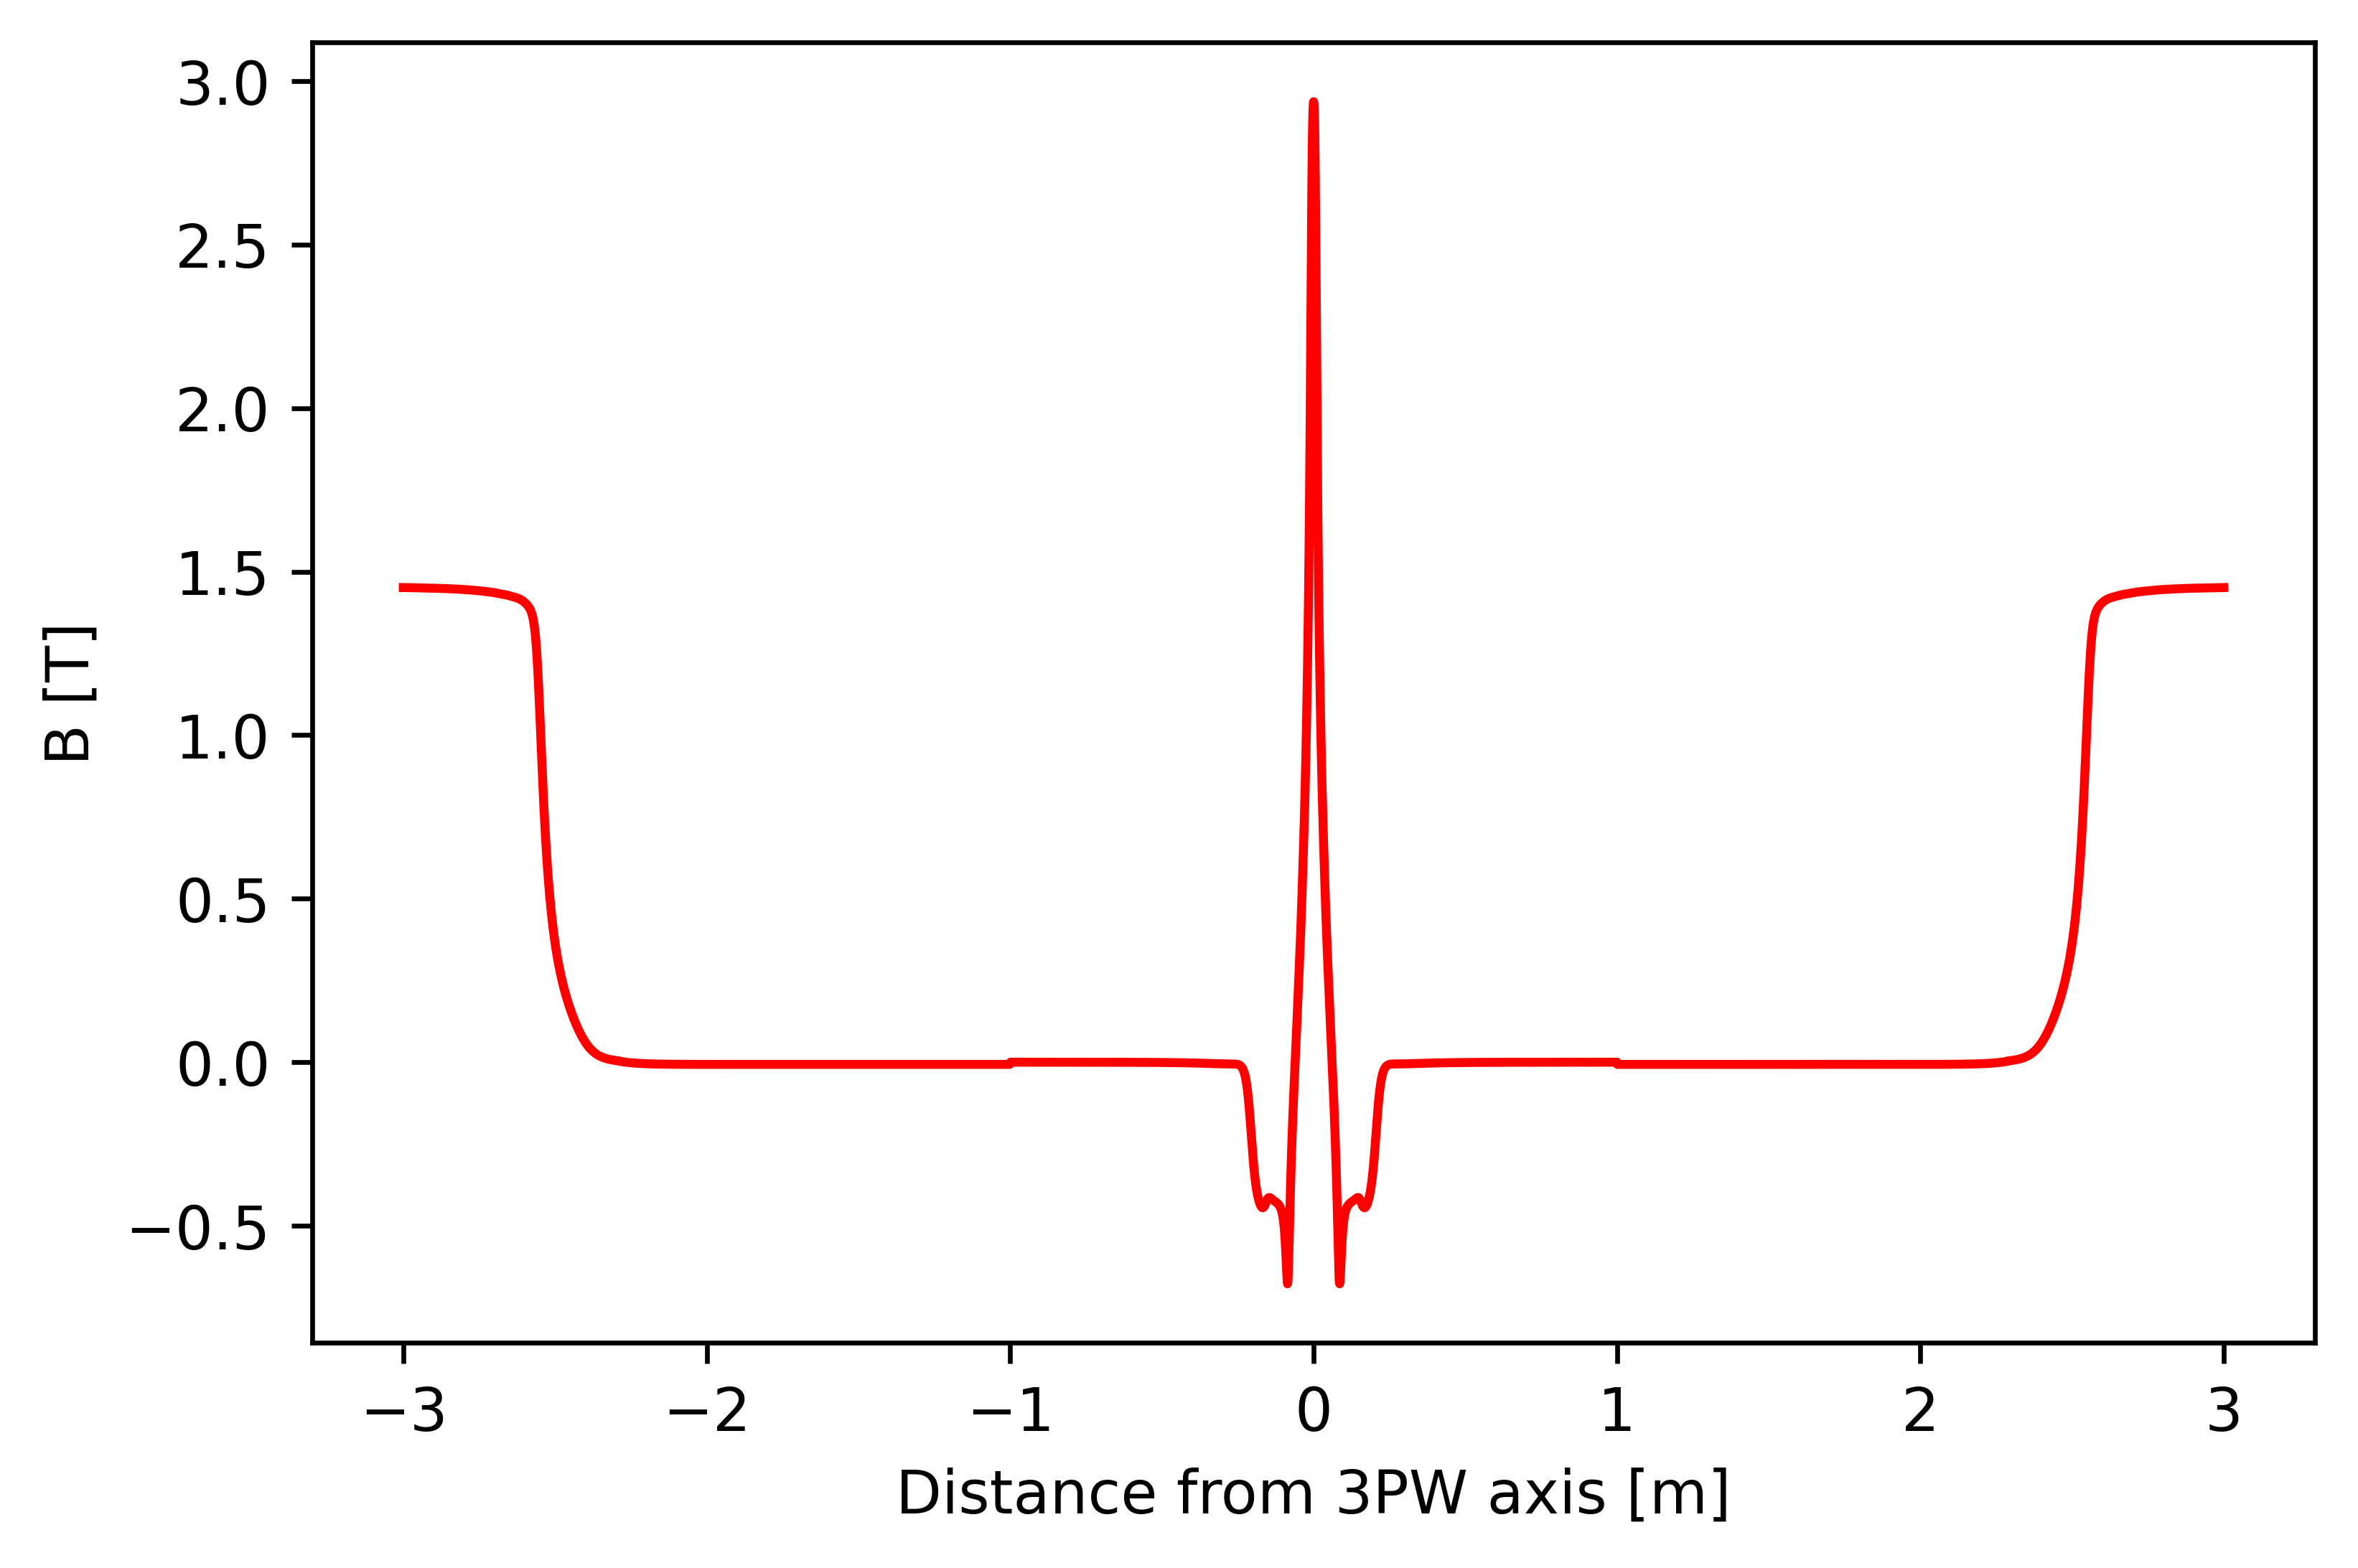
\includegraphics[width=0.8\textwidth]{images/modified_field_profile.png}
\caption{\label{fig:modifiedfieldprofile} Magnetic field profile modified considering the BEATS source plus two BMs (up and downstream) for calculation of the power load on the crotch absorber.}
\end{figure}